% ----------------------------------------------------------------------

\chapter{\textbf{Fundamentação Teórica}} % Este comando é utilizado para criar capítulos
\sloppy % Corrige estouro de linhas

\section{TECNOLOGIA NA EDUCAÇÃO}

O termo ``tecnologia'' diz respeito a muitas outras coisas além das máquinas. O conceito tecnologia engloba a criatividade engenhosa do cérebro humano desde os primórdios da Humanidade. Sua aplicação perpassa pela utilização de diversos recursos naturais, com objetivo de criar ferramentas instrumentais e simbólicas, para transpor barreiras impostas pela natureza até aos testes e aplicação de novas teorias e princípios científicos \cite{kenski2007educaccao}.

A sociedade contemporânea está inserida no momento de constante advento tecnocientífico, e de forma direta e indireta, isto reflete nas práticas pedagógicas escolares. Conforme \citeonline{martins2010gestao}, o educador deve estar sempre atualizado, pois a transformação nos processos tecnológicos e meios de comunicação são permanentes. A presença das TIC (tecnologias de informação e comunicação) na educação é um tema dinâmico e catalisador de transformações no processo ensino-aprendizagem. Estudos demonstram que a condição para o uso com êxito das TIC nas escolas reside, antes de tudo, em saber com utilizá-las e aplicá-las nas atividades curriculares \cite{noeth2004evaluating}. Nesse sentido, a qualificação profissional para o uso das TIC é primordial \cite{david2008padroes}.

De acordo com \citeonline{kenski2007educaccao}, a abordagem didática com integração das TIC no processo ensino-aprendizagem pode alavancar a aprendizagem e o desenvolvimento dos educandos via inserção digital. O grande desafio para escola e educadores, consiste em saber aplicar as TIC como potencializador no sistema educacional, especialmente em seus componentes pedagógicos e processos de ensino-aprendizagem \cite{libaneoorganizacao}.

\subsection{PLATAFORMAS DE AUXÍLIO}

No âmbito da educação, várias ferramentas têm sido utilizadas como método de auxílio na aprendizagem, bem como na aproximação do aluno com a escola. Tais instrumentos promovem novas possibilidades de interação didático pedagógica, permitindo a troca e a disponibilização de informações de forma ágil e funcional entre alunos e docentes \cite{franciscato2008avaliaccao}.

Nesta perspectiva, os \textit{Learning Management Systems} (LMS), ou ambientes virtuais de aprendizagem (AVAs), têm se mostrado grandes aliados, oferecendo desde funcionalidades de intermediação no compartilhamento de conteúdo a amplos recursos de gestão do ensino e gerenciamento administrativo \cite{tori2018educaccao}.

\begin{figure}[h]
	\caption{Perspectiva Didático Pegagógica do uso de AVAs.}
	\centering % para centralizarmos a figura
	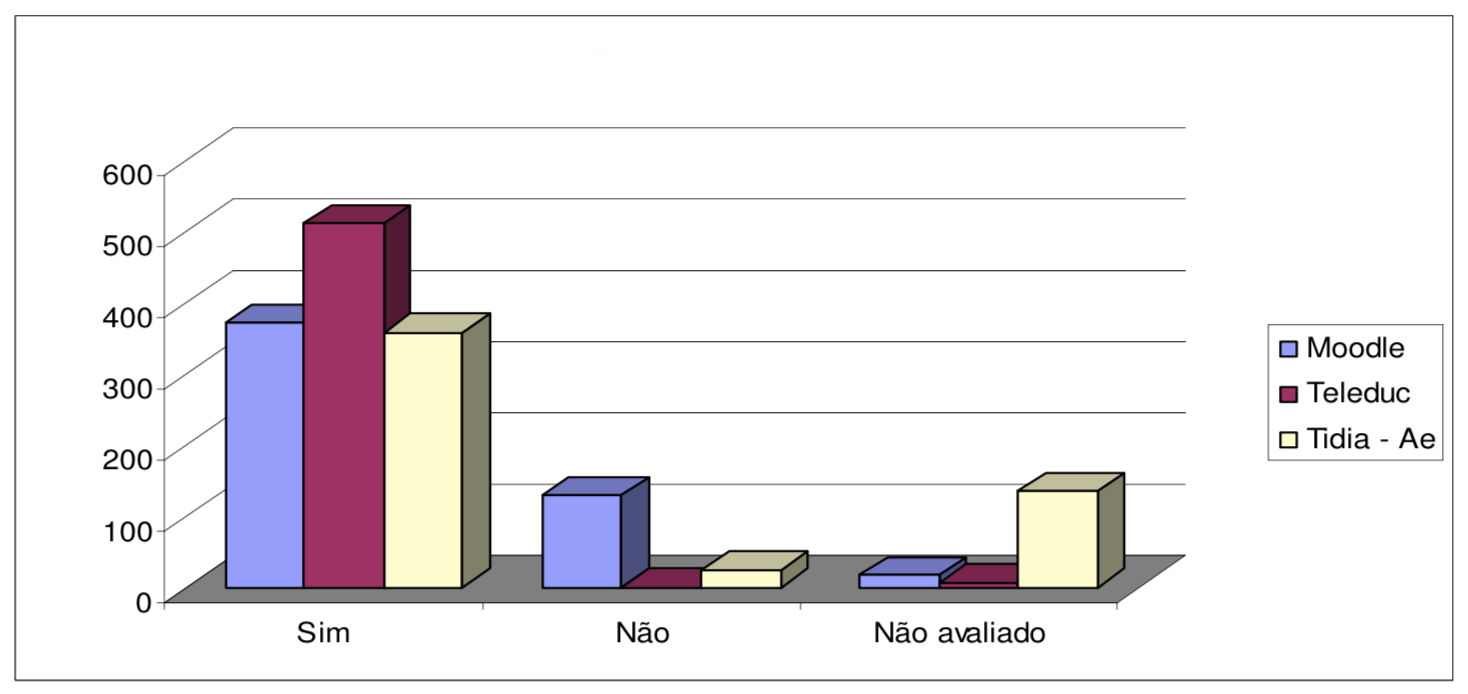
\includegraphics[width=15cm]{resources/grafico1.png} % leia abaixo
	\label{figura:perspectiva}	
	\caption*{Fonte: \citeonline{franciscato2008avaliaccao}.}
\end{figure}

A figura \ref{figura:perspectiva} demonstra o resultado de um estudo realizado para a avaliar a relevância do ponto de vista didático pedagógico de três ambientes de aprendizagem virtual: Moodle, Teleduc e Tidia - Ae. Nesta temática, procurou-se classificar os resultados em três categorias: ``Sim'' (possui relevância), ``Não'' (não possui relevância) e ``Não avaliado'' (se o participante não possui conhecimento para avaliar).

De acordo com \citeonline{sabbatini2005}, ambientes tais como \textit{Moodle} são amplamente difundidos entre escolas e universidades, constituindo extrema contribuição na metodologia de ensino. Seu foco é centralizado no aluno, sendo o papel do professor de auxílio na construção do aprendizado acadêmico. Como plataforma de ensino e gestão de aprendizagem \cite{legoinha2006moodle}, o ambiente \textit{Moodle} dispõe de várias funcionalidades, dentre elas:
\begin{itemize}
	\item Acesso a arquivos e links externos;
	\item Chat (batepapo);
	\item Fórum de discussão;
	\item Questionários de avaliação;
	\item Tarefas, testes e exercícios;
	\item Glossário;
	\item Calendário de eventos;
\end{itemize}

%\apud{saboia2013uso}{medeiroseducaccao}

%\apudonline{saboia2013uso}{medeiroseducaccao}

% \subsubsection{MOODLE}

\section{REDES NEURAIS ARTIFICIAIS}

\subsection{CONCEITO}

\citeonline{haykin2009neural} descreve o conceito de Redes Neurais Artificiais (RNA) utilizando-se do exemplo dos sistemas biológicos naturais, que possuem alta capacidade de aprendizado e conseguem assimilar informações complexas no ambiente ao redor em um curto espaço de tempo. Isto se dá pelo fato de que um computador processa informações de forma diferente de um cérebro humano, por exemplo. Neste escopo, uma rede neural objetiva o mapeamento de tais informações de forma a torná-las acessíveis para utilização, tal como afirma \citeonline[p. 28]{haykin2007redes}:

\begin{citacao}
	Uma rede neural é um processador maciçamente paralelamente distribuído constituído de unidades de processamento simples, que têm a propensão natural para armazenar conhecimento experimental e torná-lo disponível para o uso. Ela se assemelha ao cérebro em dois aspectos:
	\begin{enumerate}[leftmargin=4.7cm, topsep=0cm]
	    \item O conhecimento é adquirido pela rede a partir de seu ambiente através de um processo de aprendizagem.
	    \item Forças de conexão entre neurônios, conhecidas como pesos sinápticos, são utilizadas para armazenar o conhecimento adquirido.
	\end{enumerate}
\end{citacao}

Para \citeonline{hagan1996neural}, apesar de as as Redes Neurais não apresentarem uma solução para todos os problemas matemáticos e de engenharia, elas tem se mostrado um recurso poderoso em casos apropriados para sua aplicação. Muitos dos seus avanços atuais se devem ao avanço do poder de processamento dos computadores, o que possibilita a realização de testes cada vez mais complexos.

\subsection{MODELO DE ORGANIZAÇÃO}

Considerando o modelo de organização de uma Rede Neural Artificial (RNA), existem duas características básicas que a definem, sendo estas sua arquitetura e seu modelo de aprendizagem. Para que uma RNA funcione, se faz necessário um treinamento prévio através de dados de exemplo fornecidos, que serão levados como parâmetro para uma classificação de resultados. Neste sentido, através dos parâmetros obtidos, são atribuídos pesos para cada tipo de informação de entrada a ser processada pela rede \cite{thomas2019}.

O neurônio artificial, definido por \citeonline{mcculloch1943logical}, representa uma unidade de processamento de uma RNA, sendo de considerada de importância fundamental para o funcionamento da rede \cite{haykin2007redes}. A primeira aplicação prática de um neurônio artificial foi concebida por \citeonline{rosenblatt1958perceptron} com a rede \textit{perceptron}, capaz de realizar reconhecimento de padrões.

\begin{figure}[h]
	\caption{Modelo de neurônio artificial de McCulloch e Pitts.}
	\centering % para centralizarmos a figura
	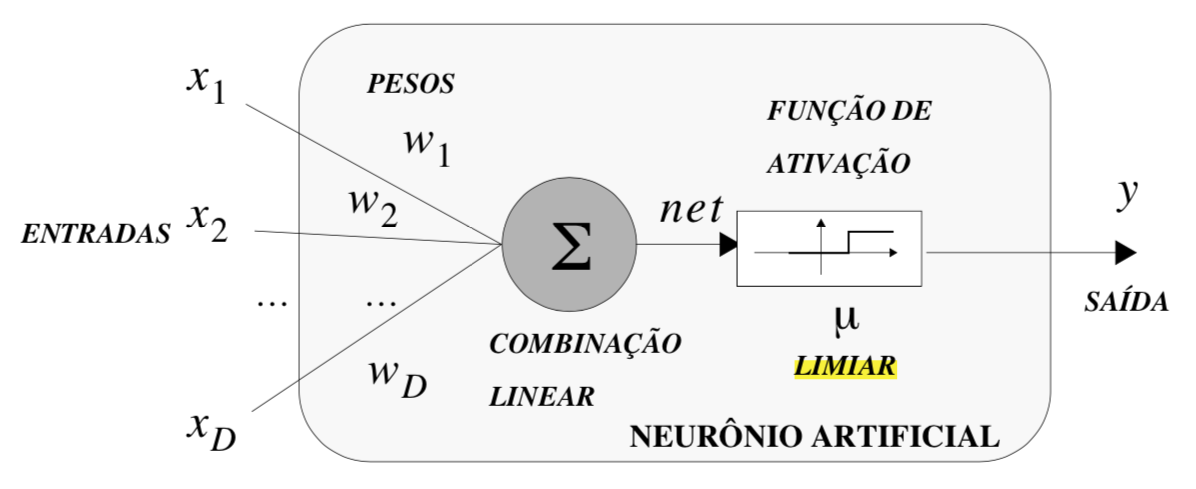
\includegraphics[width=14cm]{resources/modelo_neuronio.png} % leia abaixo
	\label{figura:modelo_neuronio}	
	\caption*{Fonte: \citeonline{thomas2019}.}
\end{figure}

A figura \ref{figura:modelo_neuronio} representa o modelo de um neurônio artificial, constituído de entradas predefinidas (x\textsubscript{1}, x\textsubscript{2}, x\textsubscript{D}), que têm o seu valor multiplicado por um peso (w\textsubscript{1}, w\textsubscript{2}, w\textsubscript{D}), indicando o grau de importância da respectiva entrada. Tais valores são somados através de uma combinação linear e encaminhados em seguida para uma função de ativação. A partir de então, é verificado se o valor produzido pela função atinge um limiar \(\mu\). Caso o resultado ultrapasse o limiar definido, o neurônio produz uma saída positiva \cite{thomas2019}.

\subsection{SINGLE LAYER PERCEPTRON X MULTILAYER PERCEPTRON}

Quanto a organização de uma Rede Neural Artificial, \citeonline{fausett1994fundamentals} descreve os arranjos de RNA's em camadas. Uma RNA com apenas uma camada é denominada uma \textit{Single Layer Perceptron}, ao passo que uma RNA com múltiplas camadas é denominada uma \textit{Multilayer Perceptron}.

\begin{figure}[h]
	\caption{Exemplo de separação linear binária.}
	\centering % para centralizarmos a figura
	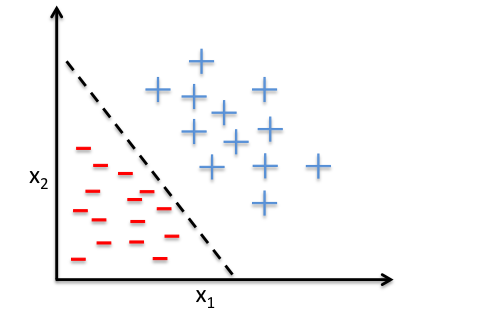
\includegraphics[width=14cm]{resources/perceptron_binary.png} % leia abaixo
	\label{figura:perceptron_binary}	
	\caption*{Fonte: \citeonline{2015_singlelayer}.}
\end{figure}

O uso de RNA's do tipo \textit{Single Layer Perceptron} se remete a problemas de ordem linear \cite{haykin2009neural}, como apresenta a figura \ref{figura:perceptron_binary}, onde duas classes de informações (+ e -), podem ser separadas por uma única reta. Tais problemas permitem a classificação de dados de entrada em até duas categorias, limitando sua aplicação à problemas mais complexos, o que pode exigir aplicação de uma rede multicamada (\textit{Multilayer Perceptron}) \cite{fausett1994fundamentals}.

Em uma rede Multilayer Perceptron, tal como representado na figura \ref{figura:multilayer_perceptron}, o emprego de várias camadas é utilizado para possibilitar a separação de elementos que uma rede Single Layer Perceptron não é capaz de realizar. Neste modelo, os perceptrons utilizam-se de funções de ativação não-lineares, que tornam possível tal refinamento no processo \cite{marius2009}.

\begin{figure}[h]
	\caption{Exemplo de separação linear não-binária.}
	\centering % para centralizarmos a figura
	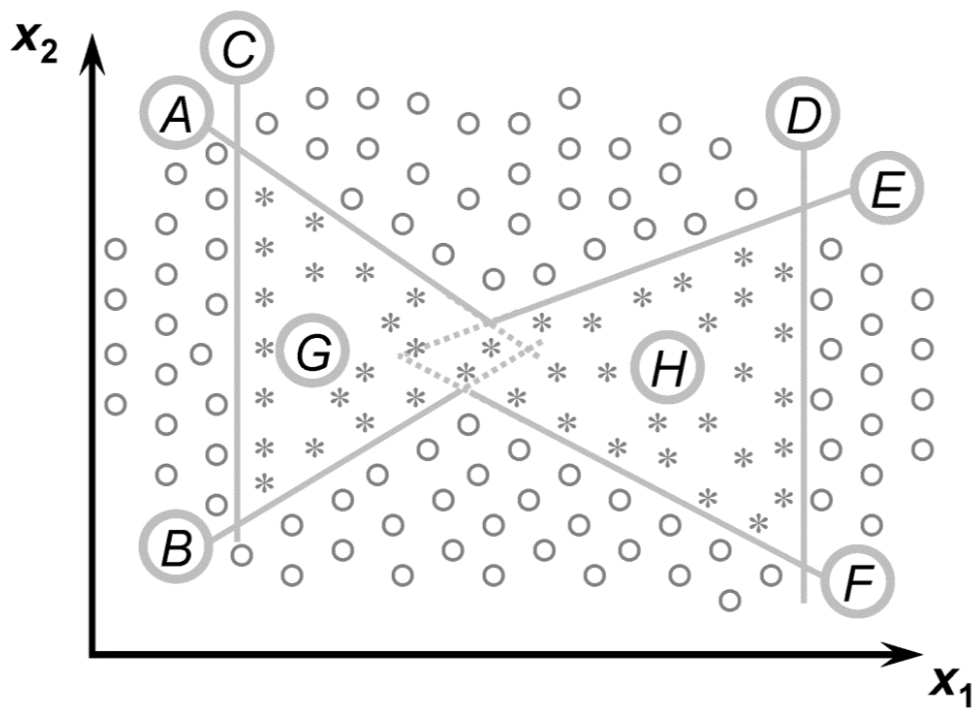
\includegraphics[width=12cm]{resources/multilayer_perceptron.png} % leia abaixo
	\label{figura:multilayer_perceptron}	
% 	\caption*{Fonte: .}
\end{figure}

\subsection{APRENDIZAGEM SUPERVISIONADA}

Quanto ao processo de aprendizagem de uma RNA, os métodos de aprendizagem podem ser classificados como supervisionados e não-supervisionados \cite{haykin2007redes}. Na ocasião do procedimento supervisionado, há um ambiente de treinamento contendo modelos de saída já conhecidos e classificados, utilizados como parâmetro para classificação \cite{marius2009}.

\citeonline{2014_supervised_learning} exemplifica a aprendizagem supervisionada descrevendo um sistema de filtragem de \textit{spam}, no qual ao visualizar um \textit{e-mail} uma pessoa saberia identificá-lo como uma mensagem de lixo eletrônico. A partir de então, seria possível reunir informações características de mensagens do mesmo tipo para classificar outras mensagens ainda não visualizadas.

Em RNA's com modelo de aprendizagem não-supervisionado, ao contrário do modelo supervisionado, não são utilizados modelos explícitos de saída para o treinamento, e nenhuma avaliação da mesma é realizada \cite{von2005rede}. Neste caso, a própria rede deve identificar os modelos de aprendizagem e criar novos, caso necessário \cite{becker1991}.

\section{TECNOLOGIAS EMPREGADAS}

\subsection{SISTEMAS DISTRIBUÍDOS}

Na computação moderna vários sistemas computacionais interagem entre si de forma interdependente, sendo a internet o exemplo mais perceptível a ser citado. São várias redes interconectadas e aplicações que fazem uso de tais estruturas para se comunicarem, abrangendo os mais variados domínios. Todas essas estruturas empregam conceitos da tecnologia sistemas distribuídos \cite{puder2011distributed}.\\
\citeonline{tanenbaum2007distributed} descrevem um sistema distribuído como sendo um conjunto de computadores autônomos não obrigatoriamente equivalentes, interligados entre si e compreendidos pelo usuário como um único sistema conexo. Sua compreensão destaca a interdependência e a colaboração entre os computadores como sendo um elemento de suma importância para a existência da arquitetura. A definição proposta por \citeonline[p. 2]{coulouris2005distributed} torna ainda mais precisa através da seguinte definição sobre sistemas distribuídos:

\begin{citacao}
	Definimos um sistema distribuído como aquele no qual os componentes de hardware ou software, localizados em computadores interligados em rede, comunicam-se e coordenam suas ações apenas enviando mensagens entre si.
\end{citacao}

\citeonline{puder2011distributed} destacam vários benefícios dos sistemas distribuídos em comparação com sistemas centralizados, tais como redundância, economia, escalabilidade e tolerância a falhas.

\subsection{WEB SERVICES}

Considerando as várias utilidades dos sistemas distribuídos, \citeonline{fielding2000} definiu em sua tese de doutorado o \textit{REpresentational State Transfer} (REST), um estilo arquitetônico para sistemas hipermídia distribuídos. Tal arquitetura foi desenvolvida com base na disponibilização de recursos, mapeados de forma exclusiva através de URIs (\textit{Uniform Resource Identifiers}), que são acessadas através de URLs (\textit{Uniform Resource Location}), funcionando sobre o protocolo HTTP \cite{richardson2008restful}. Em seu trabalho, Fielding destaca seis atribuições básicas que caracterizam o padrão REST, são estas:

\begin{enumerate}
	\item {A aplicação deve utilizar a arquitetura cliente-servidor;}
	\item {Todas as requisições devem ser independentes e isoladas entre si, não havendo nenhum estado de sessão guardado no servidor (\textit{Stateless});}
	\item {Requisições já executadas previamente podem ser mantidas em memória para reutilização futura por chamadas equivalentes (Cache);}
	\item {Deve existir uma padronização na manipulação, no mapeamento dos componentes disponibilizados e no formato de troca de dados (Interface Uniforme);}
	\item {O sistema deve ser projetado em camadas, de modo que a interação entre componentes de diferentes camadas seja limitada ao essencial;}
	\item {Código sob demanda, permitindo que \textit{applets} ou \textit{scripts} sejam baixados para execução no lado cliente (podendo ser opcional a implementação deste quesito);}
\end{enumerate}

O padrão definido por Fielding se mostra uma alternativa altamente performática em comparação com  \textit{web services} tradicionais tais como SOAP, principalmente pelo tamanho de mensagens e tempos de resposta menores, tal como afirmam \citeonline{hamad2010} e \citeonline{dudhe2014performance}. A comunidade web e grandes empresas tais como Google e Amazon têm se utilizado dessa tecnologia para construir seus serviços, dado sua simplicidade e escalabilidade \cite{wagh2014hybrid}. REST tem sido amplamente utilizado em conjunto com o \textit{JavaScript Object Notation} (JSON), uma estrutura de dados simples e leve, em substituição ao formato XML como padrão representativo de troca de dados, sendo suportado pela maioria dos \textit{Web Browsers} atuais \cite{knutsen2018}.

\begin{figure}[h]
	\caption{Arquitetura de um \textit{Web Service RESTful}.}
	\centering % para centralizarmos a figura
	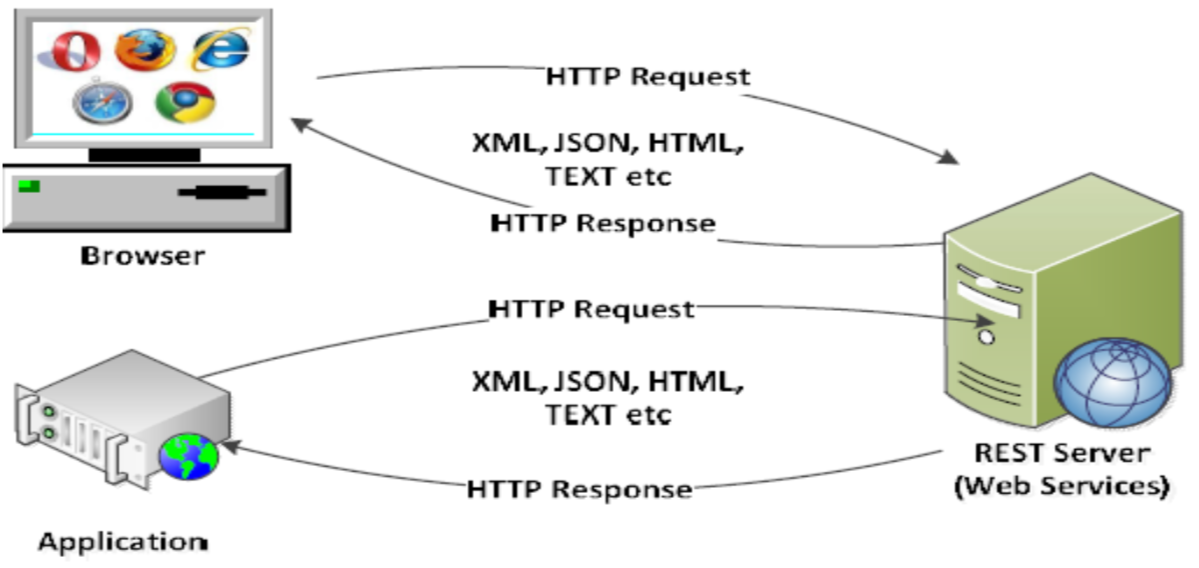
\includegraphics[width=12cm]{resources/webservices.png} % leia abaixo
	\label{figura:webservices}	
	\caption*{Fonte: \citeonline{thu2015}.}
\end{figure}

A figura \ref{figura:webservices} ilustra uma representação básica de um \textit{Web Service RESTful} implementado utilizando a arquitetura Rest (RESTful), onde essencialmente são realizadas requisições (HTTP Request) a partir de um determinado cliente (aplicação ou \textit{web browser}) para um servidor (\textit{REST Server}), que responde à solicitação com uma resposta (HTTP Response), contendo em seu corpo uma informação padronizada por algum formato representativo de troca de dados (XML, JSON, HTML, TEXT).

\begin{table}[h]
	\captionsetup{justification=centering}
	\centering
	\caption{Métodos HTTP e suas funções correspondentes.}
	\label{tabela:metodoshttp}
	\begin{tabular}{r|lr}
		Método HTTP &  Ação\\
		\hline
		GET & Lê um recurso  \\
		POST & Cria um recurso  \\
		PUT & Altera um recurso \\
		DELETE & Deleta um recurso 
	\end{tabular}
	\caption*{Fonte: \citeonline{hamad2010}.}
\end{table}

Aplicações RESTful utilizam-se dos chamados métodos HTTP para manipulação de dados. A tabela \ref{tabela:metodoshttp} lista os principais métodos e suas respectivas ações, sendo elas leitura, criação, alteração e deleção de dados, respectivamente \cite{pautasso2008restful}.

\subsection{JSON WEB TOKEN (JWT)}

Quanto à segurança de acesso, \textit{web services} RESTful podem se utilizar de mecanismos para garantir que somente usuários autorizados tenham acesso aos recursos. Neste sentido, o padrão JWT (\textit{JSON Web Token}) \cite{jwt} se mostra uma alternativa concreta para a transmissão de informações confidenciais de autenticação em sistemas \textit{stateless} \cite{jones2015json}. \citeonline{peyrott2016jwt} descreve tal padrão como um meio simples, compacto e seguro de realizar solicitações, sendo utilizado por uma grande parcela de aplicativos. O fato de se utilizar da estrutura JSON se deve a sua ampla adoção pelos  navegadores web modernos \cite{jones2011emerging}.

\begin{figure}[h]
	\caption{Estrutura básica de um token JWT.}
	\label{figura:jwt}
	\begin{center}
		\textcolor{red}{xxxxxx}.\textcolor{green}{yyyyyyy}.\textcolor{blue}{zzzzzzzz}\\
		\textcolor{red}{header}.\textcolor{green}{payload}.\textcolor{blue}{signature}\\
	\end{center}
	\caption*{Fonte: \citeonline{rahmatulloh2018}.}
\end{figure}

A figura \ref{figura:jwt} ilustra a estrutura básica do JWT, constituída basicamente por uma string de caracteres criptografada denominada Token, dividida em três seções: \textit{header}, \textit{payload} e \textit{signature}.

\citeonline{janoky2018} ressaltam algumas vantagens da utilização de \textit{tokens} JWT, justificando seu uso como forma de controle de acesso a determinadas funções em um sistema distribuído. Destacam-se dentre estas a diminuição da complexidade na utilização do serviço, e o ganho em performance, dado que todas as informações de autenticação e autorização do usuário são inseridas junto ao \textit{token}, o que dispensa a realização de uma chamada ao \textit{web service} para verificar se o usuário logado possui ou não permissão de acesso à uma determinada função.

\newpage

\begin{figure}[h]
	\caption{Diagrama de autenticação e validação de \textit{token}.}
	\centering % para centralizarmos a figura
	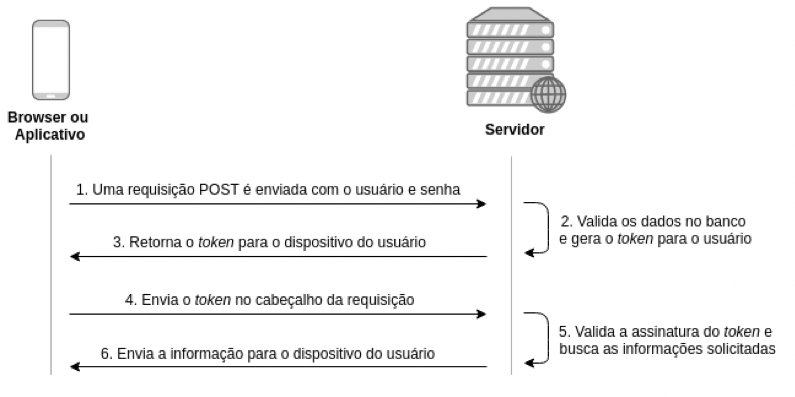
\includegraphics[width=14cm]{resources/jwt-schema.png} % leia abaixo
	\label{figura:jwt-schema}	
	\caption*{Fonte: \citeonline{montanheiro2017utilizaccao}.}
\end{figure}

Na figura \ref{figura:jwt-schema} temos um esquema básico de autenticação e validação de um \textit{token} JWT onde, na fase de autenticação, são encaminhados os dados de login do usuário para o servidor. Caso a validação tenha ocorrido com sucesso, um \textit{token} é gerado e retornado para a aplicação cliente (\textit{Browser} ou Aplicativo), que pode acessar recursos permitidos enquanto o mesmo estiver válido.

